%############################################################################
\chapter{\AutoProof Tutorial}
\label{sec:ap-tutorial}
\chapterimage{images/tutorial}
%############################################################################


\AutoProof is an auto-active\footnote{\AutoProof tries to achieve an intermediate degree of automation in the continuum that goes from \emph{auto}matic to inter\emph{active}.} verifier for the Eiffel programming language; it proves functional correctness of Eiffel programs annotated with contracts. The goal of this tutorial is to show how to verify Eiffel programs with \AutoProof through hands-on exercises.

%===========================================================
\subsection*{Preparations}
%===========================================================

To use \AutoProof locally you can install EVE on your machine. Although it is possible to use the online version of \AutoProof to do the verification exercises, some options are not available on the web.

You can download the EVE delivery at
\begin{center}
\url{http://se.inf.ethz.ch/research/eve/builds}
\end{center}

Downloads for the examples and exercises as well as links to using the web interface of \AutoProof are available here:
\begin{center}
\url{http://se.inf.ethz.ch/research/autoproof/tutorial}
\end{center}


%===========================================================
\subsection*{Structure}
%===========================================================

Each of the following sections describes in detail the use of \AutoProof based on increasingly complex examples. Each example is used throughout one section to explain some of the concepts behind \AutoProof and how they are used to verify programs. Each section also has hands-on exercises with verification tasks for one or more programs.

%############################################################################
\section{Verification of Basic Properties}
%############################################################################

To prove functional correctness automatically, a program needs a machine-readable specification. We are using Eiffel---an object-oriented programming language--- which allows one to write contracts as part of the program. Each Eiffel routine is equipped with pre- and postconditions and each class has a class invariant.

We will use the \emph{Account} example to show the basic concepts of \AutoProof. The example consists of the two classes \e{ACCOUNT} and \e{ACCOUNT_TEST}. The first class models a bank account and the second class consists of two test cases that show proper and improper usage of the class. The full code of class \e{ACCOUNT} is shown in Figure~\ref{code:account}. 

First you can look through the example and verify the two classes; all routines, except for the deliberately failing test case, will be successfully verified.

\begin{figure}
\begin{tabular}{ll}
{\begin{erunning}[basicstyle=\scriptsize,numbers=left]
note
	description: "Account class."
	model: balance, credit_limit

class ACCOUNT
create make

feature {NONE} -- Initialization

	make
			-- Initialize empty account.
		note
			status: creator
		do
			balance := 0
			credit_limit := 0
		ensure
			balance_set: balance = 0
			limit_set: credit_limit = 0
		end

feature -- Access

	balance: INTEGER
			-- Balance of this account.

	credit_limit: INTEGER
			-- Credit limit of this account.

	available_amount: INTEGER
			-- Amount available on this account.
		note status: functional
		do
			Result := balance + credit_limit
		end

feature -- Element change

	set_credit_limit (limit: INTEGER)
			-- Set `credit_limit' to `limit'.
		require
			valid: limit >= (0).max(-balance)
			modify_model ("credit_limit", Current)
		do
			credit_limit := limit
		ensure
			limit_set: credit_limit = limit
		end
\end{erunning}}
&
\hspace{3mm}
{\begin{erunning}[basicstyle=\scriptsize,numbers=left,firstnumber=last]

	deposit (amount: INTEGER)
			-- Deposit `amount' in this account.
		require
			amount_non_negative: amount >= 0
			modify_model ("balance", Current)
		do
			balance := balance + amount
		ensure
			balance_set: balance = old balance + amount
		end

	withdraw (amount: INTEGER)
			-- Withdraw `amount' from this account.
		require
			amount_not_negative: amount >= 0
			amount_available: amount <= available_amount
			modify_field (["balance", "closed"], Current)
		do
			balance := balance - amount
		ensure
			balance_set: balance = old balance - amount
		end

feature -- Basic operations

	transfer (amount: INTEGER; other: ACCOUNT)
			-- Transfer `amount' from this to `other'.
		require
			amount_not_negative: amount >= 0
			amount_available: amount <= available_amount
			no_aliasing: other /= Current
			modify (Current, other)
		do
			balance := balance - amount
			other.deposit (amount)
		ensure
			balance = old balance - amount
			other.balance = old other.balance + amount
			credit_limit = old credit_limit
			other.credit_limit = old other.credit_limit
		end

invariant
	limit_not_negative: credit_limit >= 0
	balance_not_credit: balance >= -credit_limit

end
\end{erunning}}
\end{tabular}
\caption{Account example.}
\label{code:account}
\end{figure}


%===========================================================
\subsection{Input Language}
%===========================================================

%----------------------------------------------
\subsubsection*{Eiffel Programs and Contracts}
%----------------------------------------------

Here we give a short overview of the Eiffel programming language based on the \emph{Account} example.

\paragraph{Class definition}

Eiffel is object-oriented. Classes are defined with the \e{class} keyword. If no inheritance clause is given (as in this example), then the class implicitly inherits from the class \e{ANY}, which serves as a common ancestor for all classes.

\begin{erunning}
class
	ACCOUNT
\end{erunning}

\paragraph{Constructors}

To define constructors for the class, you can use the \e{create} keyword, followed by a comma-separated list of constructors called \emph{creation routines}. If no constructor is defined, the routine \e{default_create} will implicitly become the only creation routine. In our example the routine \e{make} will be the creation procedure.

\begin{erunning}
create
	make
\end{erunning}

\paragraph{Features and visibility}

Routines and attributes (together called \emph{features}) are defined in feature blocks using the \e{feature} keyword. Feature blocks can declare a visibility restriction by indicating a list of class names in curly braces. For example the first feature block restricts the access of the make routine to \e{NONE}, essentially hiding the routine from all other classes (no class can inherit from \e{NONE}). The other feature blocks do not have any access restriction and thus the features inside these feature blocks are public. It is common to name feature clauses by adding a comment using the double-dash \e{--} comment style (there are no multi-line comments in Eiffel).

\begin{erunning}
feature {NONE} -- Initialization
feature -- Access
feature -- Basic operations
\end{erunning}

\paragraph{Attributes}

Attributes are defined with an attribute name followed by the type of the attribute. For all features it is common to add a comment on the line following the feature declaration.

\begin{erunning}
	balance: INTEGER
		-- Balance of this account.
\end{erunning}

\paragraph{Routines}

A routine declaration consists of the routine name, optional parameters, optional return type, optional precondition, routine body and optional postcondition. The precondition denoted by the \e{require} keyword and postcondition denoted by the \e{ensure} keyword are the specification of the routine. The precondition holds prior to the execution of the routine, and the postcondition holds afterwards. Therefore the precondition is the responsibility of the client of the routine, whereas the postcondition has to be established by the routine itself. If a pre- or postcondition is omitted, the routine will have an implicit pre- or postcondition of \e{True}.

\begin{erunning}
	set_credit_limit (limit: INTEGER)
			-- Set `credit_limit' to `limit'.
		require
			valid: limit >= (0).max(-balance)
			modify_model ("credit_limit", Current)
		do
			credit_limit := limit
		ensure
			limit_set: credit_limit = limit
		end
\end{erunning}

\paragraph{Assertion tags}

Each assertion, be it a precondition, a postcondition, a class or loop invariant, or an intermediate check instruction, can have an \emph{assertion tag}. These tags are useful for debugging, as the feedback from \AutoProof will specify the tag of violated assertions.

\paragraph{Class invariants}

Class invariants are written at the end of a class using the \e{invariant} keyword. Class invariants define the state of a consistent object and hold by default whenever an object is visible to other classes, for example at the beginning and end of each public routine.

\begin{erunning}
invariant
	credit_limit_not_negative: credit_limit >= 0
	balance_not_below_credit: balance >= -credit_limit
\end{erunning}

There are more details on how to write an Eiffel program and what specification can be written for the verification with \AutoProof; this will be explained throughout the rest of the tutorial.

%----------------------------------------------
\subsubsection*{\AutoProof Annotations}
%----------------------------------------------

\AutoProof supports tow forms of custom annotations: note clauses for features and classes, and dummy routines made available through \e{ANY}.

Note clauses are used to denote special types of routines and attributes that influence the verification like creation routines (see Section~\ref{sec:creator}) or ghost features (see Section~\ref{sec:ghost}). Additionally, note clauses are used to disable defaults for implicit pre-/postconditions of the ownership methodology (see Section~\ref{sec:wrapping}). %and~\ref{sec:semicola}).

The second form of \AutoProof annotations are dummy features (routines and functions with empty implementation) that can be used in assertions or regular code. These features are defined in class \e{ANY} and are available everywhere. \AutoProof gives special semantics to these features, for example to specify modifies clauses (see Section~\ref{sec:framing}).

You can look at the \AutoProof manual for a complete listing of custom annotations of both note clauses and dummy features\footnote{\url{http://se.inf.ethz.ch/research/autoproof/manual/\#annotations}}.

%===========================================================
\subsection{Basic Properties}
%===========================================================

%----------------------------------------------
\subsubsection*{Booleans}
%----------------------------------------------

The Eiffel boolean operations \e{not}, \e{and}, \e{or}, \e{xor}, and \e{implies} are supported by \AutoProof. The semi-strict operators \e{and then} and \e{or else} are also supported with the correct semantics that the right-hand side only needs to be valid if the left-hand side does not already define the overall value of the expression.

%----------------------------------------------
\subsubsection*{Integers}
%----------------------------------------------

The Eiffel integer operations \e{+}, \e{-}, \e{*}, \e{//} (quotient of integer division), and \e{\\\\} (remainder of integer division) are supported by \AutoProof. Integers in \AutoProof can be modeled in two modes, either as mathematical integers or as machine integers. By default integers will be modeled as mathematical integers, though \AutoProof can also check overflows of bounded integers (see Section~\ref{sec:overflow}).

The Eiffel comparison operations on integers \e{=}, \e{/=}, \e{<}, \e{>}, \e{<=}, and \e{>=} are all supported.

%----------------------------------------------
\subsubsection*{References}
%----------------------------------------------

Comparison of objects always uses reference equality. The standard equality operator \e{a = b} and inequality operator \e{a /= b} work as expected; object equality \e{a ~ b} and inequality \e{a /~ b} are not supported and will fall back to reference equality when used.

%===========================================================
\subsection{Models}
%===========================================================

\AutoProof supports \emph{model-based contracts}. Models are used to express the \emph{abstract state space} of a class and describe its changes. To define the model of a class you add a \e{model} annotation to the \e{note} clause of the class. The model may only consist of attributes of the class.

\begin{SCfigure}[50][!h]
\begin{erunning}
note
	model: balance, credit_limit
class ACCOUNT ...
\end{erunning}
\hspace{0.5cm}
\caption*{This makes the two attributes \e{balance} and \e{credit_limit} model fields of the class.}
\end{SCfigure}

The idea behind model-based contracts is to have an abstract and concise yet expressive way to specify the interface of a class. When using models you use the class invariant to describe object validity in terms of the model attributes. The effect of each procedure is expressed by relating the pre-state of the model fields to their post-state. In addition you can express the framing specification in terms of the model fields.

The Mathematical Model Library (MML, see Section~\ref{sec:mml}) can be used to model complex behavior. Also, ghost attributes might be introduced to define abstract behavior in terms of other functions or attributes and can then be used as model fields (see Section~\ref{sec:ghost}).

%\todo{expand? add example?}

%===========================================================
\subsection{Framing} \label{sec:framing}
%===========================================================

The framing model that \AutoProof uses is based on \emph{modifies clauses}. The \e{ACCOUNT} class deliberately used three different ways of specifying the modifies clause to demonstrate the differences between them.

\subsubsection*{\e{modify_model (fields, objects)}}

Using \e{modify_model} you can specify that model fields may change during the execution of a routine. You can specify one or more model fields by providing as first parameter a manifest string with the name of the model attribute or a manifest tuple with multiple manifest strings. The second parameter is either a single object, a single set of objects of type \e{MML_SET}, or a manifest tuple with mixed objects or sets of objects.

\begin{SCfigure}[50][!h]
\begin{erunning}
deposit (amount: INTEGER)
	require
		...
		modify_model ("balance", Current)
	do ... end
\end{erunning}
\hspace{0.5cm}
\caption*{This routine is allowed to modify the model field \e{balance} of the \e{Current} object.}
\end{SCfigure}

The effect of \e{modify_model} is as follows: each model attribute specified in the \e{modify_model} clause \emph{as well as each non-model attribute} can be modified in the routine. All model fields that are not listed remain unchanged. This means in turn that for clients all non-model attributes are potentially modified even though they are not listed in the modifies clause.

\subsubsection*{\e{modify_field (fields, objects)}}

With \e{modify_field} you specify directly which attributes may be changed by a routine. As before,
you can specify one or more attribute names by providing as first parameter a manifest string with the name of the model attribute or a manifest tuple with multiple manifest strings. The second parameter is again either a single object, a single set of objects of type \e{MML_SET}, or a manifest tuple with mixed objects or sets of objects.

\begin{SCfigure}[50][!h]
\begin{erunning}
withdraw (amount: INTEGER)
	require
		...
		modify_field (["balance", "closed"], Current)
	do ... end
\end{erunning}
\hspace{0.5cm}
\caption*{This routine is allowed to modify the attributes \e{balance} and \e{closed} of the \e{Current} object.}
\end{SCfigure}

This way of specifying the modifies clause is lower-level than specifying which model fields may change. This is also the reason we are required to add the ghost field \e{closed} in the example shown here. The \e{closed} field is a boolean flag that is \e{True} whenever an object is in a consistent state (see Section~\ref{sec:ownership} for details).

\subsubsection*{\e{modify (objects)}}

The third option to specify modifies clauses is to give a list of objects which can be modified without limiting the modifications to certain attributes or model fields. For this modifies clause you can specify mixed objects or sets of objects.

\begin{SCfigure}[50][!h]
\begin{erunning}
transfer (amount: INTEGER; other: ACCOUNT)
	require
		...
		modify (Current, other)
	do ... end
\end{erunning}
\hspace{0.5cm}
\caption*{This routine is allowed to modify all attributes of \e{Current} and \e{other}.}
\end{SCfigure}

Since the objects may be modified freely, you have to specify the full effect on the modified objects. For example the \e{transfer} procedure of the account example, the postcondition not only describes the effect on the \e{balance} attribute of the two objects but also has clauses to specify that the \e{credit_limit} attribute does not change. This is for demonstration purposes only, it would be a better design to use \e{modify_model} instead (\emph{try to change it!}).

Giving an empty tuple as argument---\e{modify ([])}---denotes that nothing may be modified, i.e., that the routine is \emph{pure}.

\subsubsection*{Default Modifies Clauses}

When no modifies clause is given a default modifies clause is used based on the type of routine:
\begin{itemize}
\item For \textbf{procedures} (routines without a return value), the default modifies clause is \e{modify (Current)}. So all attributes can be modified in a procedure if no specific modifies clause is given.
\item For \textbf{functions} (routines with a return value), the default modifies clause is \e{modify ([])}. Therefore, by default, all functions are \emph{pure}.
\end{itemize}

When you overwrite the default modifies clause for procedures, for example to modify an object passed as parameter, and you want to be able to modify the \e{Current} object as well, you will need to add \e{modify (Current)} to the modifies clause (or a more specific version when only a subset of the attributes needs to be modifiable).

\subsubsection*{Combining modifies annotations}

You can add several modifies annotations to a modifies clause. The set of modifiable objects and attributes is the union of all modifies annotations.

%===========================================================
\subsection{Routine Annotations}
%===========================================================

%----------------------------------------------
\subsubsection*{Creation Procedures} \label{sec:creator}
%----------------------------------------------

Creation procedures can be used as regular routines as well. Therefore, \AutoProof will verify all creation routines twice, once as creation routines and once as regular routines. The context of the verification is different for the two verifications, as for example for creation routines all attributes are initialized to their default values before the routine is executed.

You can instruct \AutoProof to verify a creation routine only once by adding a \e{creator} annotation. This denotes the routine as being creation-only and \AutoProof will not verify it as a regular routine.

\begin{SCfigure}[50][!h]
\begin{erunning}
make
	note
		status: creator
	do ... end
\end{erunning}
\hspace{0.5cm}
\caption*{Marks \e{make} to be only a creation routine.}
\end{SCfigure}

%----------------------------------------------
\subsubsection*{Functional Functions}
%----------------------------------------------

\AutoProof supports a special type of function, consisting of only a single assignment to \e{Result}. To declare such a function you have to add a \e{functional} annotation to the function. These functions are defined by their implementation and have an implicit postcondition; given an implementation \e{Result := x} the implicit postcondition will be \e{Result = x}.

\begin{SCfigure}[50][!h]
\begin{erunning}
available_amount: INTEGER
	note
		status: functional
	do
		Result := balance + credit_limit
	end
\end{erunning}
\hspace{0.5cm}
\caption*{Marks \e{available_amount} to be \emph{functional}, therefore only consisting of a single assignment to \e{Result}.}
\end{SCfigure}


%===========================================================
\subsection{Debugging Verification}
%===========================================================

The only feedback given by \AutoProof is whether a routine is successfully verified or if some specific assertions could not be proven. When the verification fails it can be necessary to find out which facts the verifier could establish or even guide the verifier to the right conclusion. For this you can use intermediate assertions (\e{check} instructions in Eiffel). During the debugging process it can also be beneficial to \emph{assume} specific facts and thus limit the possible executions that the verifier considers during the proof.

%----------------------------------------------
\subsubsection*{Assertions}
%----------------------------------------------

Using Eiffel's \e{check} instruction you can add an intermediate assertion that will be verified by \AutoProof. This can help to check if you have the same understanding of the state at a program point as the verifier. You can add multiple expressions to a single check instruction, and each expression can be equipped with a tag. \AutoProof will show the tags in error messages.

\begin{SCfigure}[50][!h]
\begin{erunning}[numbers=none]
check tag: expr end
\end{erunning}
\hspace{0.5cm}
\caption*{Check instruction to establish if \e{expr} holds.}
\end{SCfigure}

Note that it is possible that when you have multiple consecutive assertions successfully verified, removing an intermediate assertion will make the verification of later assertions fail. In these cases you have to keep the assertion in order to guide the verifier towards the successful verification.

%----------------------------------------------
\subsubsection*{Assumptions}
%----------------------------------------------

Eiffel does not support assumptions out of the box. To write an assumption in \AutoProof, you have to write a check instruction with the special tag \e{assume}. \AutoProof will assume the expression for the rest of the routine without checking it.

You can use assumptions to limit the executions considered by the verifier. For example by assuming \e{False} in a branch of a conditional instruction the verification of that branch will always succeed.

\begin{SCfigure}[50][!h]
\begin{erunning}
if ... then
	...
else
	check assume: False end
end
\end{erunning}
\hspace{0.5cm}
\caption*{Ignores all code path that go through the \e{else} branch.}
\end{SCfigure}

Another way to use assumptions to limit executions it by restricting the state space of otherwise unrestricted values. This can be used for example to ignore executions where an array is empty.

\begin{SCfigure}[50][!h]
\begin{erunning}[numbers=none]
check assume: not a.is_empty end
\end{erunning}
\hspace{0.5cm}
\caption*{Ignores executions where \e{a} is empty.}
\end{SCfigure}

%----------------------------------------------
\subsubsection*{Inconsistencies}
%----------------------------------------------

It can happen that verification succeeds due to inconsistent contracts or assumptions. If you for example have a routine with the precondition \e{a > 0} and an additional class invariant \e{a < 0} (or an assumption \e{a < 0} in the body of the routine), your specification is inconsistent. This is essentially equivalent to an assumption of \e{False} and the verifier will be able to derive any fact from it, including false ones.

A quick (though not completely safe) check for inconsistencies is to add an assertion or postcondition \e{False} to your routine. If the verifier manages to prove the assertion, this is a sign for an inconsistency in the specification.


%===========================================================
\subsection{Hands-On: Clock}
%===========================================================

The \e{CLOCK} class is modeling a clock counting seconds, minutes and hours of a day. The class contains routines to create the clock, set the time, and increase the time.

\begin{enumerate}[label=\bfseries Task \arabic*:, leftmargin=1.8cm]
\item Add a \e{model} declaration to define the abstract model.
\item Add a class \e{invariant} to restrict the attribute values.
\item Add a precondition to the creation procedure \e{make}. \\ 
      You should be able to verify \e{make} and \e{test_make}.
\item Add the specification to the \e{set_*} procedures. \\ 
      You should be able to verify the \e{set_*} and \e{test_set} procedures.
\item Add the specification to the \e{increase_*} procedures. \\
      You should be able to verify both classes completely.
\end{enumerate}


%############################################################################
\newpage
\section{Verification of Algorithmic Problems}
%############################################################################

An important aspect in the verification of programs is verifying algorithms. In this section we will focus on the verification of algorithmic problems on arrays, such as searching and sorting. The concepts needed to verify array algorithms are also necessary for other types of algorithms.

We use the algorithm of finding the maximum element of an integer array as an example. The code is shown in Figure~\ref{code:max_in_array}. You can look through the example again and verify it. In the rest of this section we will explain in detail how one verifies such an algorithm.

\begin{figure}[!h]
\begin{adjustwidth}{-10pt}{-10pt}
\begin{erunning}[basicstyle=\footnotesize,numbers=left]
class MAX_IN_ARRAY
feature -- Basic operations

	max_in_array (a: SIMPLE_ARRAY [INTEGER]): INTEGER
			-- Find the maximum element of `a'.
		require
			array_not_empty: a.count > 0
		local 
			i: INTEGER
		do
			Result := a[1]
			from
				i := 2
			invariant
				i_in_bounds: 2 <= i and i <= a.sequence.count + 1
				max_so_far: across 1 |..| (i-1) as c all a.sequence[c.item] <= Result end
				in_array: across 1 |..| (i-1) as c some a.sequence[c.item] = Result end
			until
				i > a.count
			loop
				if a[i] > Result then
					Result := a[i]
				end
				i := i + 1
			variant
				a.count - i
			end
		ensure
			is_maximum: across 1 |..| a.count as c all a.sequence[c.item] <= Result end
			in_array: across a.sequence.domain as c some a.sequence[c.item] = Result end
		end

end
\end{erunning}
\end{adjustwidth}
\caption{\emph{Maximum in array} example.}
\label{code:max_in_array}
\end{figure}

%===========================================================
\subsection{Mathematical Model Library} \label{sec:mml}
%===========================================================

To express complex mathematical properties, \AutoProof supports the \emph{Mathematical Model Library}. This library consists of classes modeling sets, bags (or multisets), sequences, maps, intervals, and relations. You can find an API description of these classes online\footnote{\url{http://se.inf.ethz.ch/research/autoproof/reference/}}.

MML classes do not have an implementation and should therefore only ever be used for specifications (using \emph{ghost fields} and \emph{ghost code} as discussed in Section~\ref{sec:ghost}). They have an efficient axiomatization in the back-end verifier, and are therefore well suited to be used with \AutoProof.

%----------------------------------------------
\subsubsection*{MML Types}
%----------------------------------------------

The most important MML types are:
\begin{itemize}
\item \e{MML_SET [G]}: A set contains distinct objects. Each element can only be contained once and the order is irrelevant.
\item \e{MML_SEQUENCE [G]}: A sequence is an ordered list of elements. Indexing starts at 1.
\item \e{MML_BAG [G]}: A bag (or multiset) is a set where each element can appear multiple times. The order of elements is irrelevant.
\end{itemize}

%----------------------------------------------
\subsubsection*{Shorthand Notations}
%----------------------------------------------

Several shorthand notations exist to declare sets and sequences making the use of MML classes easier.
\begin{itemize}
\item Sets of type \e{MML_SET [ANY]} can be declared using the Eiffel manifest tuple notation: \e{s := [a, b]}.
\item Sets of type \e{MML_SET [G]} can be declared using the Eiffel manifest array notation: \e{s := <<a, b>>}.
\item Sequences of type \e{MML_SEQUENCE [G]} can be declared using the Eiffel manifest array notation: \e{s := <<a, b>>}.
\item Use \e{\{MML_SET [G]\}.empty_set} to declare an empty set.
\item Use \e{\{MML_SEQUENCE [G]\}.empty_sequence} to declare empty sequences.
\end{itemize}

For the last two shorthands it is not possible to use the empty array notation \e{<< >>} due to the intricacies of Eiffel typing.

%===========================================================
\subsection{\e{SIMPLE_ARRAY} and \e{SIMPLE_LIST}}
%===========================================================

When you want to use arrays or lists in verification, you need classes that have a fully specified interface. The classes from EiffelBase do not offer this, therefore when verifying algorithms with \AutoProof, you should use the two provided classes \e{SIMPLE_ARRAY [G]} and \e{SIMPLE_LIST [G]}. Both classes have a ghost model field \e{sequence} of type \e{MML_SEQUENCE [G]} and all features are specified in terms of the model. You can find an API description of these classes online\footnote{\url{http://se.inf.ethz.ch/research/autoproof/reference/}}.

To make it easier for \AutoProof to deal with specifications involving these classes you should use the \e{sequence} model field when writing complex assertions involving the container contents. For example the loop invariant of the \e{max_in_array} function is written as:
\begin{erunning}
2 <= i and i <= a.sequence.count + 1
across 1 |..| (i-1) as c all a.sequence[c.item] <= Result end
across 1 |..| (i-1) as c some a.sequence[c.item] = Result end
\end{erunning}
Were you to replace \e{a.sequence} with just \e{a}, \AutoProof would not verify the routine anymore (\emph{try it!}).

%===========================================================
\subsection{Quantifiers}
%===========================================================

Eiffel supports bounded universal and existential quantifiers with the \e{across} expression. In our example, where we find the maximum in an array, we can use this to express the desired postcondition that all elements in the array are smaller or equal to the result. Universal quantification is done using the \e{across..all} expression. With the Eiffel interval expression \e{1 \|..\| a.count} we can quantify over all integers between (and including) \e{1} and \e{a.count}. 

\begin{erunning}[numbers=none]
across 1 |..| a.count as c all a.sequence[c.item] <= Result end
\end{erunning}

The across loop uses a cursor, therefore we have to use \e{c.item} to access the current element of the iteration. For the correctness of the algorithm we also have to express that the result is an element of the array, not just larger than all elements. We can do this with an existential quantification using Eiffel's \e{across..some} loop.

\begin{erunning}[numbers=none]
across a.sequence.domain as c some a.sequence[c.item] = Result end
\end{erunning}

In the last example we used the \e{domain} query for the quantification to show that you can use different approaches to reach the same goals. This query defined in \e{MML_SEQUENCE} returns a set of integer values that contains all index values of the sequence and is therefore equivalent to using an interval from \e{1} to \e{a.count} (all MML sequences are indexed from 1).

\AutoProof supports the following domains for quantification:
\begin{itemize}
\item Integer intervals. The quantified variable will be of type \e{INTEGER}.
\item Sets of type \e{MML_SET [G]}. The quantified variable will be of type \e{G}.
\item Sequences of type \e{MML_SEQUENCE [G]}. The quantified variable will be of type \e{G}. This is equivalent to quantifying over the \e{range} of a sequence.
\item Objects of type \e{SIMPLE_ARRAY [G]} or \e{SIMPLE_LIST [G]}. The quantified variable will be of type \e{G}. This is equivalent to quantifying over the \e{sequence} of the array or list.
\end{itemize}

%===========================================================
\subsection{Termination}
%===========================================================

\AutoProof will verify termination of loops and direct recursive calls (indirect recursion is not checked). To prove termination you can define \emph{loop variants} for loops or \emph{decreases clauses} for loops and recursive routines.

%----------------------------------------------
\subsubsection*{Loop Variant}
%----------------------------------------------

The loop variant is an integer expression that is non-negative and decreases with each loop iteration. This implies that the loop can only be executed a finite number of times.

\begin{SCfigure}[50][!h]
\begin{erunning}
loop ...
variant
	a.count - i
end
\end{erunning}
\hspace{0.5cm}
\caption*{The loop variant decreases each loop iteration and stays non-negative.}
\end{SCfigure}

\AutoProof infers loop variants of simple loops. For example a loop with exit condition \e{a > b} will have an inferred loop variant of \e{b - a}. In the example in Figure~\ref{code:max_in_array} specifying the variant is not necessary.

%----------------------------------------------
\subsubsection*{Decreases Clause}
%----------------------------------------------

In complex algorithms it is possible that an integer value is not enough to express the loop variant. For these cases \AutoProof supports \e{decreases} clauses. A decreases clause can contain multiple arguments of type \e{INTEGER}, \e{MML_SET}, or \e{MML_SEQUENCE}. The semantics of a decreases clause is that in each loop iteration the tuple that contains all the elements of the decreases clause needs to become lexicographically smaller while remaining bounded from below. The lower bound is 0 for integers and is the empty set or empty sequence for sets and sequences.

The decreases clause for a loop is written in the loop invariant.

\begin{SCfigure}[50][!h]
\begin{erunning}
from ...
invariant
	decreases (a.count - i)
until ...
\end{erunning}
\hspace{0.5cm}
\caption*{Decreases clause equivalent to the previous loop variant.}
\end{SCfigure}

For recursive functions the decreases clause is added to the precondition. Otherwise it behaves like the decreases clause for loops: at each recursive call the value of the decreases clause must become smaller while remaining bounded.

\begin{SCfigure}[50][!h]
\begin{erunning}
f (a: SET [INTEGER]; b: INTEGER)
	require
		decreases (a, b)
	do ... end
\end{erunning}
\hspace{0.5cm}
\caption*{Decreases clause of a recursive function.}
\end{SCfigure}

%----------------------------------------------
\subsubsection*{Non-termination}
%----------------------------------------------

Sometimes it is not desirable to prove termination of an algorithm. For these cases you can add an empty decreases clause to the loop or recursive function and \AutoProof will skip the termination check.

\begin{SCfigure}[50][!h]
\begin{erunning}
from ...
invariant
	decreases ([])
until ...
\end{erunning}
\hspace{0.5cm}
\caption*{A possibly non-terminating loop.}
\end{SCfigure}

%===========================================================
\subsection{Hands-On: Linear and Binary Search}
%===========================================================

With the knowledge we have so far we now verify algorithms searching an element in an array. These algorithms do not change the array and are therefore \emph{pure}, thus simplifying the specification.

%----------------------------------------------
\subsubsection*{Linear Search}
%----------------------------------------------

\begin{enumerate}[label=\bfseries Task \arabic*:, leftmargin=1.8cm]
\item Add the loop variant to verify that the loop terminates. \\
      You should be able to verify \e{linear_search} in its current form.
\item Add postconditions to \e{linear_search} to verify the test class. \\
      You should be able to verify the test class.
\item Add loop invariants to verify the postcondition. \\
      You should be able to verify both classes completely.
\end{enumerate}

%----------------------------------------------
\subsubsection*{Binary Search}
%----------------------------------------------

\begin{enumerate}[label=\bfseries Task \arabic*:, leftmargin=1.8cm]
\item Add loop invariants to verify that all array accesses are valid.
\item Add the loop variant to verify that the loop terminates. \\
      You should be able to verify \e{binary_search} in its current form.
\item Add precondition to require input arrays to be sorted.
\item Add postconditions to \e{binary_search} to verify the test class. \\
      You should be able to verify the test class.
\item Add loop invariants to verify the postcondition. \\
      You should be able to verify both classes completely.
\end{enumerate}

%----------------------------------------------
\subsubsection*{Recursive Binary Search}
%----------------------------------------------

\begin{enumerate}[label=\bfseries Task \arabic*:, leftmargin=1.8cm]
\item Add the specification to \e{binary_search} (you can reuse the specification of the iterative version). \\
      You should be able to verify the test class.
\item Add precondition to \e{binary_search_recursive_step} to require the input array to be sorted and to verify that all array accesses are valid.
\item Add a decreases clause to to prove termination of the recursion. \\
      You should be able to verify \e{binary_search_recursive_step} in its current form.
\item Add postconditions to \e{binary_search_recursive_step} to verify the algorithm. \\
      You should be able to verify both classes completely. \\
      \textbf{Note: you might need intermediate assertions to verify the postcondition.}
\end{enumerate}


%===========================================================
\newpage
\subsection{Ghost State and Ghost Functions} \label{sec:ghost}
%===========================================================

The next examples---iterative and recursive binary search---have preconditions that the input array is sorted. Writing an expression that expresses this property directly in the precondition can become unwieldy. It is beneficial to write helper functions that capture such properties with a meaningful name and that allow reuse of the function.

The \emph{sorted} property was expressed over the \emph{sequence} of the array, which is of type \e{MML_SEQUENCE}. As mentioned before (see Section~\ref{sec:mml}), MML types are not executable and can only be used for specification purposes. We call code that is used only for specification purposes \emph{ghost code}; ghost code is never executed and only interpreted by the verifier.

To write expressive specifications \AutoProof supports ghost code in the form of \emph{ghost functions}, using \emph{ghost attributes}, and writing \emph{lemmas}. Ghost code should never influence executable code, therefore assignments from ghost code to regular attributes is not allowed. \AutoProof does \textbf{not} enforce this currently, so using ghost code outside specifications may lead to undefined behavior.

%----------------------------------------------
\subsubsection*{Ghost Functions}
%----------------------------------------------

Ghost functions are useful to write helper functions usable in specifications, for example to express that a sequence is sorted. To mark a function as \emph{ghost} you add a \e{note} clause with \e{status: ghost}. If the function is also \emph{functional}, the note clause can be shortened by combining the two \e{status} properties.

\begin{erunning}
is_sorted (s: MML_SEQUENCE [INTEGER]): BOOLEAN
		-- Is `s' sorted?
	note
		status: functional, ghost
	do
		Result := across 1 |..| s.count as i all
		            across 1 |..| s.count as j all
		              i.item <= j.item implies s[i.item] <= s[j.item] end end
	end
\end{erunning}

With ghost function like the one shown above we can simplify contracts and promote reuse of specification constructs, for example in iterative and recursive binary search (\emph{try it!}).

%----------------------------------------------
\subsubsection*{Ghost State}
%----------------------------------------------

Ghost state is introduced by having \emph{ghost attributes}. These attributes can be used like regular attributes in contracts, frame conditions, code, and as model fields. Most commonly you would use ghost attributes to define model fields that are then related to existing attributes or other objects through class invariants and other contracts. A linked list could for example represents its contents in form of a sequence using a ghost attribute to store the sequence and then declaring this attribute to be a model field.

To declare a ghost attribute you need to add a \e{note} clause to the attribute. The Eiffel syntax for doing this is the following:

\begin{erunning}
sequence: MML_SEQUENCE [INTEGER]
	note status: ghost
	attribute
	end
\end{erunning}

%----------------------------------------------
\subsubsection*{Lemmas}
%----------------------------------------------

Intermediate assertions are not always sufficient for difficult proofs. In these cases you can use \emph{lemma} procedures to support verification. Calling a lemma procedure has the same effect as calling other procedures: the verifier asserts the precondition and assumes the postcondition. Lemmas can therefore be used to add $A(x)\implies B(x)$ to the fact space, where $A(x)$ is the precondition and $B(x)$ is the postcondition of the lemma.

Lemmas are implicitly \emph{ghost} and \emph{pure}. You declare a lemma using a special \e{note} clause.
\begin{erunning}
lemma (x)
	note status: lemma
	require
		$A (x)$
	do
		-- Proof that A(x) implies B(x)
	ensure
		$B (x)$
	end
\end{erunning}

Lemmas are proven like a regular procedures. You might need to \emph{implement} a proof; sometimes you can use recursion in a lemma which is akin to an induction proof.

%===========================================================
\subsection{Accessing Pre-state}
%===========================================================

Eiffel allows the use of \e{old} expressions in postcondition to express the effect of a routine in relation to the pre-state. This syntax is limited, as it cannot be used in \e{across} expressions or in the body of the routine (e.g. in loop invariants).

\AutoProof offers an extension to the \e{old} mechanism through a ghost query \e{old_} defined in \e{ANY}. This query can be used anywhere in the code or in the postcondition to reference the value of an expression in the pre-state of the routine.

\begin{SCfigure}[50][!h]
\begin{erunning}[numbers=none]
check s.old_[i] = s[i] end
\end{erunning}
\hspace{0.5cm}
\caption*{Assertion that item \e{s [i]} is unchanged.}
\end{SCfigure}

%===========================================================
\subsection{Integer Overflows} \label{sec:overflow}
%===========================================================

\AutoProof can check a program for integer overflows. By default overflow checking is disabled. You can enable it among \AutoProof's options or, if you use the command line version, with the \e{-overflow} command line option.

%===========================================================
\subsection{Hands-On: Sorting}
%===========================================================

The next examples are about sorting of arrays. The algorithms shown here are in-place algorithms that operate on the array directly. As a preliminary exercise we look at the notion of permutation of arrays and how to express this in \AutoProof.

%----------------------------------------------
\subsubsection*{Permutation}
%----------------------------------------------

\begin{enumerate}[label=\bfseries Task \arabic*:, leftmargin=1.8cm]
\item Find the correct encoding of permutation (only one is correct).
\item For each incorrect encoding try to find two sequences that successfully pass the check instruction while not being real permutations.
\end{enumerate}

%----------------------------------------------
\subsubsection*{Gnome Sort}
%----------------------------------------------

\begin{enumerate}[label=\bfseries Task \arabic*:, leftmargin=1.8cm]
\item Add the frame specification, pre- and postcondition to \e{gnome_sort}. \\
      Add implementation of \e{is_part_sorted}. \\
      You should be able to verify the test class.
\item Add loop invariants to verify that all array accesses are valid.
\item Add loop invariants to verify the postcondition. \\
      You should be able to verify both classes completely.
\item Enable overflow checking and verity absence of overflows.
\end{enumerate}

%----------------------------------------------
\subsubsection*{Insertion Sort}
%----------------------------------------------

\begin{enumerate}[label=\bfseries Task \arabic*:, leftmargin=1.8cm]
\item Add a precondition and loop invariant to \e{insertion_sort} and the precondition to \e{swap} to verify that all array accesses are valid.
\item Add the loop variants to verify that the loops terminate. \\
      You should be able to verify \e{insertion_sort} and \e{swap} in its current form.
\item Add the postcondition to \e{insertion_sort}. \\
      You should be able to verify the test class. \\
      \textbf{You might want to introduce helper functions.}
\item Add the postcondition to \e{swap} and the necessary loop invariants to verify the postcondition. \\
      You should be able to verify both classes completely.
\item Enable overflow checking and verity absence of overflows.
\end{enumerate}


%============================================================================
\section{Object Consistency and Ownership} \label{sec:ownership}
%============================================================================

For this section we use an unbalanced binary tree as an example. Each tree node has a value and one or two children. The \e{maximum} function returns the maximum element in the tree. An excerpt of the tree node class is shown in Figure~\ref{code:tree_node}.

\begin{figure}
\begin{adjustwidth}{-4pt}{-4pt}
\begin{tabular}{ll}
{\begin{erunning}[basicstyle=\scriptsize,numbers=left]
class TREE_NODE

create
	make, make_with_children

feature {NONE} -- Initialization

	make (a_value: INTEGER)
			-- Initialize node.
		note
			status: creator
		do
			value := a_value
		ensure
			value_set: value = a_value
			no_left: left = Void
			no_right: right = Void
		end

	make_with_children (a_value: INTEGER; 
			    a_l, a_r: TREE_NODE)
			-- Initialize node.
		note
			status: creator
			explicit: contracts
		require
			a_l.is_wrapped
			a_r.is_wrapped

			modify (Current)
			modify_field ("owner",[a_l,a_r])
		do
			value := a_value
			left := a_l
			right := a_r
		ensure
			value_set: value = a_value
			left_set: left = a_l
			right_set: right = a_r
			default_is_closed: is_wrapped
		end

feature -- Access

	value: INTEGER
			-- Value of this node.
\end{erunning}}
&
\hspace{4mm}
{\begin{erunning}[basicstyle=\scriptsize,numbers=left,firstnumber=last]

	left, right: TREE_NODE
			-- Left and right node (Void if none).

feature -- Basic operations

	maximum: INTEGER
			-- Maximum value of this tree.
		require
			decreases (sequence)
		do
			Result := value
			if left /= Void then
				check owns.has (left) end
				Result := Result.max (left.maximum)
			end
			if right /= Void then
				check owns.has (right) end
				Result := Result.max (right.maximum)
			end
		ensure
			max: across sequence.domain as i all 
			              sequence[i.item] <= Result end
			exists: sequence.has (Result)
		end

feature -- Model

	sequence: MML_SEQUENCE [INTEGER]
			-- Sequence of values.
		note
			status: ghost
		attribute
		end

invariant
	owns_def: owns = {like owns}[[left,right]] / Void
	sequence_def: sequence =
		(if left = Void 
		   then {like sequence}.empty_sequence 
		   else left.sequence end) +
		{like sequence}[<<value>>] +
		(if right = Void 
		   then {like sequence}.empty_sequence 
		   else right.sequence end)
end
\end{erunning}}
\end{tabular}
\end{adjustwidth}
\caption{Excerpt of the binary tree example.}
\label{code:tree_node}
\end{figure}




%===========================================================
\subsection{State of an Object}
%===========================================================


\AutoProof uses an invariant model where objects can be in a consistent state or in a potentially inconsistent state. Consistent objects are \emph{closed} and their class invariants are guaranteed to hold. Inconsistent objects are \emph{open} and their class invariant is potentially violated. Objects can only be modified when they are open, changing the value of an attribute is not allowed when an object is closed.

\AutoProof supports a dynamic ownership model where objects can be \emph{owned} by other objects. The ownership relations can evolve during runtime. Objects that are unowned or whose owner is open are called \emph{free}. We define a shorthand for objects that are \emph{closed} and \emph{free} calling them \emph{wrapped}. When an object is in a consistent state, the ownership tree rooted in that object is guaranteed to be consistent as well.

To model the object consistency and ownership relation, each objects has a boolean ghost field \e{closed}, a ghost field \e{owner} pointing to the potential owner of the object, and a ghost field \e{owns} that contains the set of all owned objects. The relationship between the \e{owns} set and \e{owner} field is guaranteed to hold for objects in a consistent state. A special case is \e{Void} which is always \e{open}. \e{Void} can therefore never be owned and must not be part of the \e{owns} set.

\begin{figure}[!htb]
\begin{center}
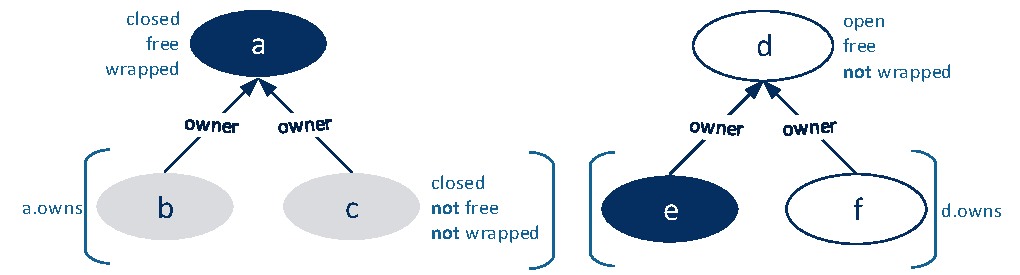
\includegraphics[width=\columnwidth]{images/objectstate.pdf}
\end{center}
\caption{Example of an object structure at run-time.} 
\label{fig:objectstate}
\end{figure}

We illustrate the possible object states on the example object structure of Figure~\ref{fig:objectstate}. The object structure consist of six objects:

\begin{itemize}
\item Object \e{a} is \emph{closed}, therefore its class invariant is guaranteed to hold. It does not have an owner and thus is \emph{free}. As it is both free and closed, it is also \emph{wrapped}. The object \e{a} owns the two objects \e{b} and \e{c}. This is defined through its \e{owns} set, i.e. \e{a.owns = \{b, c\}}.

\item Objects \e{b} and \e{c} are both owned by \e{a}, so their \e{owner} ghost field points to \e{a}. Since they are \emph{owned} they are \emph{not free}. As their owner \e{a} is \emph{closed}, the two objects \e{b} and \e{c} are \emph{closed} as well, as they are in \e{a}'s ownership domain.

\item Object \e{d} is \emph{open} and may potentially be in an inconsistent state, so its class invariant is not guaranteed to hold. It does not have an owner and is therefore \emph{free}. The object \e{d} owns the two objects \e{e} and \e{f}, defined through its \e{owns} set.

\item Object \e{e} is \emph{closed} and therefore consistent. Its owner is \e{d}, but since \e{d} is \emph{open}, \e{e} is considered to be \emph{free}. Being both \emph{closed} and \emph{free} means that \e{e} is \emph{wrapped}.

\item Object \e{f} is \emph{open} and potentially inconsistent. Analogous to \e{e} it is \emph{free}, as its owner \e{d} is \emph{open}.
\end{itemize}

The example illustrates the difference between ownership trees of \emph{open} and \emph{closed} objects. While ownership trees of consistent objects are guaranteed to be consistent as well---all objects in the ownership tree including the root object are \emph{closed}---, this property does not hold for ownership trees of potentially inconsistent objects. The ownership tree of an \emph{open} object may contain objects that are \emph{open} and objects that are \emph{closed}.


%===========================================================
\subsection{Object State Queries}
%===========================================================

\AutoProof offers ghost functions that can be used to query an object's state in assertions and specifications:

\begin{itemize}
\item \e{is_wrapped: BOOLEAN} -- is the object wrapped (closed and free)?
\item \e{is_free: BOOLEAN} -- is the object free (unowned or owner is open)?
\item \e{is_open: BOOLEAN}  -- is the object open (potentially inconsistent)?
\item \e{closed: BOOLEAN} -- is the object closed (consistent)?
\item \e{owner: ANY} -- owner of the object.
\item \e{owns: MML_SET [ANY]} -- set of owned objects.
\item \e{inv: BOOLEAN} -- does full invariant of the object hold?
\item \e{inv_only (t): BOOLEAN} -- does the invariant with tag \emph{t} hold?
\item \e{inv_without (t): BOOLEAN} -- does the invariant except for tag \emph{t} hold?
\end{itemize}

The last two functions \e{inv_only} and \e{inv_without} allow to reuse specification constructs. The argument to these functions is a list of manifest strings containing invariant tags. Given the class of Figure~\ref{code:tree_node} the condition that the \e{sequence} is consistent can be written as \e{inv_only ("sequence_def")}. This helps reduce the annotation burden for classes with comples class invariants.


%===========================================================
\subsection{Encoding Ownership}
%===========================================================

Ownership in \AutoProof is used by adding objects to and removing objects from the \e{owns} set. The usual way of doing this is by defining the \e{owns} set as part of the class invariant. The binary tree example has the following class invariant:
\begin{erunning}[numbers=none]
owns_def: owns = {like owns}[[left, right]] / Void
\end{erunning}
The owns set consists of the two objects \e{left} and \e{right} unless they are \e{Void}. As in other situations, the encoding of the \e{owns} set influences the ability of \AutoProof to reason about it. In the \e{maximum} function of the binary tree we have introduced two assertions \e{owns.has (left)} and \e{owns.has (right)} in the respective branches. Where we to remove these check instructions \AutoProof would fail in verifying the function (\emph{try it!}). 

This is due to the use of the set removal operation \e{/ Void}, which makes the reasoning about the set more difficult and forces us to help the verifier in the proof. Were we to use a different encoding of the \e{owns} set in the class invariant we could remove these assertions. The following encoding is more verbose but better suited for the verifier:
\begin{erunning}[basicstyle=\footnotesize]
owns =
	if left = Void then
		if right = Void then {like owns}[[]] else {like owns}[[right]] end
	else
		if right = Void then {like owns}[[left]] else {like owns}[[left, right]] end
	end
\end{erunning}
With this encoding there is no need for the intermediate check instructions anymore (\emph{try it!}).

%===========================================================
\subsection{Wrapping and Unwrapping} \label{sec:wrapping}
%===========================================================

The two ghost procedures \e{wrap} and \e{unwrap} are used to change an object from being \emph{unwrapped} to being \emph{wrapped} and vice versa. Figure~\ref{fig:wrapunwrap} gives an overview of how the object consistency changes when these procedures are called. 

\begin{figure}[!htb]
\begin{center}
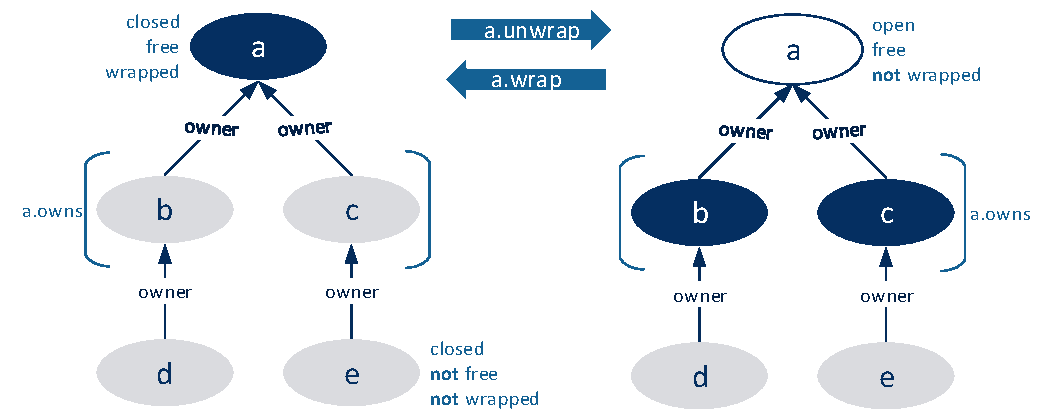
\includegraphics[width=\columnwidth]{images/wrapunwrap.pdf}
\end{center}
\caption{Change of object state on wrapping and unwrapping.}
\label{fig:wrapunwrap}
\end{figure}

Since wrapping and unwrapping changes the boolean ghost field \e{closed}, that field must be writable when either of these procedures are called. This is also the reason we had to add the field \e{closed} to the modifies clause in the \e{withdraw} procedure of the \emph{account} example (see Section~\ref{sec:framing}).

\e{wrap} and \e{unwrap} are axiomatized in the background theory of the verifier. Their definition in the class \e{ANY} does therefore not reflect their real semantics. The actual specification for \e{wrap} and \e{unwrap} could be written as follows:

\noindent\begin{tabular}{ll}
{\begin{erunning}[basicstyle=\scriptsize,numbers=left]
wrap
		-- Wrap `Current'.
	require
		is_open
		inv
		across owns as o all o.item.is_wrapped end
		modify_field ("closed", Current)
		modify_field ("owner", owns)
	ensure
		is_wrapped
		across owns as o all o.item.owner = Current end
	end
\end{erunning}}
&
\hspace{4mm}
{\begin{erunning}[basicstyle=\scriptsize,numbers=left,firstnumber=last]
unwrap
		-- Unwrap `Current.
	require
		is_wrapped
		modify_field ("closed", Current)
	ensure
		is_open
		across owns as o all 
		       o.item.is_wrapped end
	end
\end{erunning}}
\end{tabular}


%----------------------------------------------
\subsection{Defaults}
%----------------------------------------------

\AutoProof uses implicit default contracts, default wrapping, and default assignments of ghost fields to remove the annotation burden. The default contracts and wrapping depend on type and visibility of routines. The default assignment to ghost fields depends on their definition.

\paragraph{Creation routines} require by default that all arguments are wrapped. In addition, the \e{Current} object will be implicitly wrapped at the end of the routine body and the postcondition will assert that \e{Current} is wrapped.
\begin{erunning}
make ($args$)
	require
		$\forall o\in args : o$.is_wrapped
	do
		...
		Current.wrap
	ensure
		Current.is_wrapped
		$\forall o\in args : o$.is_wrapped
	end
\end{erunning}

\paragraph{Pure functions} can by default be called on \emph{closed} objects. It is therefore not necessary to unwrap the object before calling a function. Also there is no default postcondition since the objects are not mutated during the execution.
\begin{erunning}
pure_function ($args$): $type$
	require
		Current.is_closed
		$\forall o\in args : o$.is_closed
	do ...	end
\end{erunning}

\paragraph{Public procedures and public impure functions} require by default that all objects are in a consistent state, as they are callable from client code.
\begin{erunning}
public_procedure ($args$)
	require
		Current.is_wrapped
		$\forall o\in args : o$.is_wrapped
	do
		Current.unwrap
		...
		Current.wrap
	ensure
		Current.is_wrapped
		$\forall o\in args : o$.is_wrapped
	end
\end{erunning}

\paragraph{Private procedures and private impure functions} are only callable from a restricted set of clients, for example from the class itself. Since all public routines by default unwrap the \e{Current} object, private routines by default assume the object to be open.
\begin{erunning}
private_procedure ($args$)
	require
		Current.is_open
	do ...
	ensure
		Current.is_open
	end
\end{erunning}

\paragraph{Ghost fields} that have a definition in the class invariant of the form \e{$fieldname$ = $expression$} will be assigned implicitly every time the object is wrapped. This is the reason that the two ghost fields \e{owns} and \e{sequence} of the binary tree example are never explicitly assigned. \AutoProof assigns these fields implicitly at the end of each procedure when the implicit call to \e{wrap} takes place.

\paragraph{Functional functions} are often used in contracts and class invariants. Therefore they may operate on inconsistent objects and have no default preconditions.

%----------------------------------------------
\subsubsection*{Disabling Defaults}
%----------------------------------------------

It is possible to disable defaults by adding the following \e{note} clauses to routines and classes:
\begin{itemize}
\item \e{explicit: contracts} -- disable default pre- and postcondition; applicable to a routine or a class.
\item \e{explicit: wrapping} -- disable default \e{unwrap} and \e{wrap} instructions; applicable to a routine or a class.
\item \e{explicit: $\ fieldname$} -- disable default assignment to field $fieldname$ before wrapping; applicable to a class.
\end{itemize}

%===========================================================
\subsection{Modification of Owned Objects}
%===========================================================

Modifies clauses define a set of modifiable objects. Whenever an object is modifiable then the \emph{transitive closure} of all owned objects is also modifiable. It is therefore not necessary to add owned objects to a modifies clause when the owner is modifiable. A modifies clause of \e{modify (o)} is sufficient to potentially modify objects owned by \e{o}. Modifications of owned objects still require that the modified object is unwrapped.

%===========================================================
\subsection{Hands-On: Ring Buffer}
%===========================================================

The next exercise is about implementing a ring buffer backed by an array. This will highlight how to use ownership and model-based contracts to design a data structure.

\begin{enumerate}[label=\bfseries Task \arabic*:, leftmargin=1.8cm]
\item Add ownership definition for the \e{data} array to the class invariant.
\item Add class invariants for the bounds of \e{start} and \e{free}.
\item Add the model fields, model declaration, and class invariant describing the model.
\item Add the specifications to the routines of \e{RING_BUFFER}. The tests in the test class can help you to get the specification right. \\
      You should be able to verify both classes completely.
\end{enumerate}


